% AUTO-GENERATED by `python -m analysis.results` — do not edit by hand.
\documentclass[tikz,border=2pt]{standalone}
\usepackage{pgfplots}
\pgfplotsset{compat=1.17}
\begin{document}
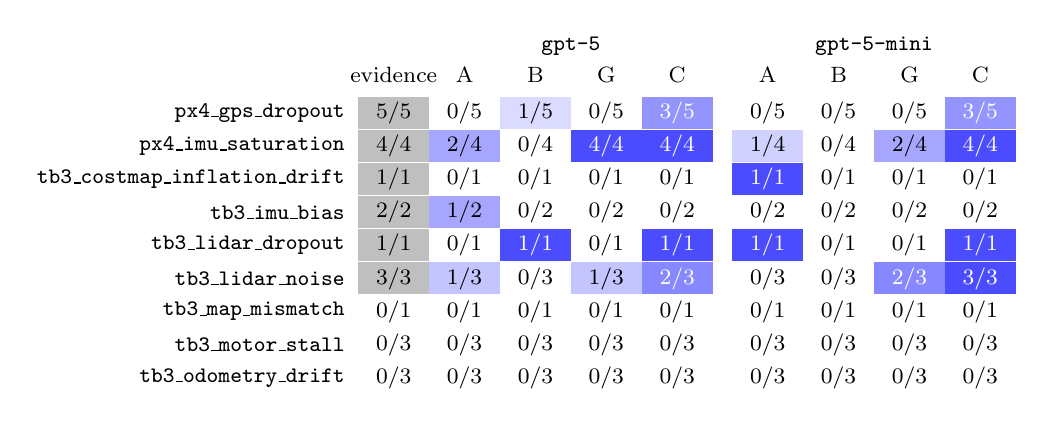
\begin{tikzpicture}[font=\footnotesize]
\node[anchor=south] at (1.35,3.83) {A};
\node[anchor=south] at (2.25,3.83) {B};
\node[anchor=south] at (3.15,3.83) {G};
\node[anchor=south] at (4.05,3.83) {C};
\node[anchor=south] at (5.20,3.83) {A};
\node[anchor=south] at (6.10,3.83) {B};
\node[anchor=south] at (7.00,3.83) {G};
\node[anchor=south] at (7.90,3.83) {C};
\node[anchor=south] at (2.70,4.18) {\texttt{gpt-5}};
\node[anchor=south] at (6.55,4.18) {\texttt{gpt-5-mini}};
\node[anchor=south] at (0.45,3.83) {evidence};
\node[anchor=east] at (-0.05,3.57) {\texttt{px4\_gps\_dropout}};
\fill[black!25] (0,3.36) rectangle (0.90,3.78);
\node at (0.45,3.57) {5/5};
\fill[blue!0!white] (0.90,3.36) rectangle (1.80,3.78);
\node[text=black] at (1.35,3.57) {0/5};
\fill[blue!14!white] (1.80,3.36) rectangle (2.70,3.78);
\node[text=black] at (2.25,3.57) {1/5};
\fill[blue!0!white] (2.70,3.36) rectangle (3.60,3.78);
\node[text=black] at (3.15,3.57) {0/5};
\fill[blue!42!white] (3.60,3.36) rectangle (4.50,3.78);
\node[text=white] at (4.05,3.57) {3/5};
\fill[blue!0!white] (4.75,3.36) rectangle (5.65,3.78);
\node[text=black] at (5.20,3.57) {0/5};
\fill[blue!0!white] (5.65,3.36) rectangle (6.55,3.78);
\node[text=black] at (6.10,3.57) {0/5};
\fill[blue!0!white] (6.55,3.36) rectangle (7.45,3.78);
\node[text=black] at (7.00,3.57) {0/5};
\fill[blue!42!white] (7.45,3.36) rectangle (8.35,3.78);
\node[text=white] at (7.90,3.57) {3/5};
\draw[white, line width=0.6pt] (0,3.36) -- (8.35,3.36);
\node[anchor=east] at (-0.05,3.15) {\texttt{px4\_imu\_saturation}};
\fill[black!25] (0,2.94) rectangle (0.90,3.36);
\node at (0.45,3.15) {4/4};
\fill[blue!35!white] (0.90,2.94) rectangle (1.80,3.36);
\node[text=black] at (1.35,3.15) {2/4};
\fill[blue!0!white] (1.80,2.94) rectangle (2.70,3.36);
\node[text=black] at (2.25,3.15) {0/4};
\fill[blue!70!white] (2.70,2.94) rectangle (3.60,3.36);
\node[text=white] at (3.15,3.15) {4/4};
\fill[blue!70!white] (3.60,2.94) rectangle (4.50,3.36);
\node[text=white] at (4.05,3.15) {4/4};
\fill[blue!18!white] (4.75,2.94) rectangle (5.65,3.36);
\node[text=black] at (5.20,3.15) {1/4};
\fill[blue!0!white] (5.65,2.94) rectangle (6.55,3.36);
\node[text=black] at (6.10,3.15) {0/4};
\fill[blue!35!white] (6.55,2.94) rectangle (7.45,3.36);
\node[text=black] at (7.00,3.15) {2/4};
\fill[blue!70!white] (7.45,2.94) rectangle (8.35,3.36);
\node[text=white] at (7.90,3.15) {4/4};
\draw[white, line width=0.6pt] (0,2.94) -- (8.35,2.94);
\node[anchor=east] at (-0.05,2.73) {\texttt{tb3\_costmap\_inflation\_drift}};
\fill[black!25] (0,2.52) rectangle (0.90,2.94);
\node at (0.45,2.73) {1/1};
\fill[blue!0!white] (0.90,2.52) rectangle (1.80,2.94);
\node[text=black] at (1.35,2.73) {0/1};
\fill[blue!0!white] (1.80,2.52) rectangle (2.70,2.94);
\node[text=black] at (2.25,2.73) {0/1};
\fill[blue!0!white] (2.70,2.52) rectangle (3.60,2.94);
\node[text=black] at (3.15,2.73) {0/1};
\fill[blue!0!white] (3.60,2.52) rectangle (4.50,2.94);
\node[text=black] at (4.05,2.73) {0/1};
\fill[blue!70!white] (4.75,2.52) rectangle (5.65,2.94);
\node[text=white] at (5.20,2.73) {1/1};
\fill[blue!0!white] (5.65,2.52) rectangle (6.55,2.94);
\node[text=black] at (6.10,2.73) {0/1};
\fill[blue!0!white] (6.55,2.52) rectangle (7.45,2.94);
\node[text=black] at (7.00,2.73) {0/1};
\fill[blue!0!white] (7.45,2.52) rectangle (8.35,2.94);
\node[text=black] at (7.90,2.73) {0/1};
\draw[white, line width=0.6pt] (0,2.52) -- (8.35,2.52);
\node[anchor=east] at (-0.05,2.31) {\texttt{tb3\_imu\_bias}};
\fill[black!25] (0,2.10) rectangle (0.90,2.52);
\node at (0.45,2.31) {2/2};
\fill[blue!35!white] (0.90,2.10) rectangle (1.80,2.52);
\node[text=black] at (1.35,2.31) {1/2};
\fill[blue!0!white] (1.80,2.10) rectangle (2.70,2.52);
\node[text=black] at (2.25,2.31) {0/2};
\fill[blue!0!white] (2.70,2.10) rectangle (3.60,2.52);
\node[text=black] at (3.15,2.31) {0/2};
\fill[blue!0!white] (3.60,2.10) rectangle (4.50,2.52);
\node[text=black] at (4.05,2.31) {0/2};
\fill[blue!0!white] (4.75,2.10) rectangle (5.65,2.52);
\node[text=black] at (5.20,2.31) {0/2};
\fill[blue!0!white] (5.65,2.10) rectangle (6.55,2.52);
\node[text=black] at (6.10,2.31) {0/2};
\fill[blue!0!white] (6.55,2.10) rectangle (7.45,2.52);
\node[text=black] at (7.00,2.31) {0/2};
\fill[blue!0!white] (7.45,2.10) rectangle (8.35,2.52);
\node[text=black] at (7.90,2.31) {0/2};
\draw[white, line width=0.6pt] (0,2.10) -- (8.35,2.10);
\node[anchor=east] at (-0.05,1.89) {\texttt{tb3\_lidar\_dropout}};
\fill[black!25] (0,1.68) rectangle (0.90,2.10);
\node at (0.45,1.89) {1/1};
\fill[blue!0!white] (0.90,1.68) rectangle (1.80,2.10);
\node[text=black] at (1.35,1.89) {0/1};
\fill[blue!70!white] (1.80,1.68) rectangle (2.70,2.10);
\node[text=white] at (2.25,1.89) {1/1};
\fill[blue!0!white] (2.70,1.68) rectangle (3.60,2.10);
\node[text=black] at (3.15,1.89) {0/1};
\fill[blue!70!white] (3.60,1.68) rectangle (4.50,2.10);
\node[text=white] at (4.05,1.89) {1/1};
\fill[blue!70!white] (4.75,1.68) rectangle (5.65,2.10);
\node[text=white] at (5.20,1.89) {1/1};
\fill[blue!0!white] (5.65,1.68) rectangle (6.55,2.10);
\node[text=black] at (6.10,1.89) {0/1};
\fill[blue!0!white] (6.55,1.68) rectangle (7.45,2.10);
\node[text=black] at (7.00,1.89) {0/1};
\fill[blue!70!white] (7.45,1.68) rectangle (8.35,2.10);
\node[text=white] at (7.90,1.89) {1/1};
\draw[white, line width=0.6pt] (0,1.68) -- (8.35,1.68);
\node[anchor=east] at (-0.05,1.47) {\texttt{tb3\_lidar\_noise}};
\fill[black!25] (0,1.26) rectangle (0.90,1.68);
\node at (0.45,1.47) {3/3};
\fill[blue!23!white] (0.90,1.26) rectangle (1.80,1.68);
\node[text=black] at (1.35,1.47) {1/3};
\fill[blue!0!white] (1.80,1.26) rectangle (2.70,1.68);
\node[text=black] at (2.25,1.47) {0/3};
\fill[blue!23!white] (2.70,1.26) rectangle (3.60,1.68);
\node[text=black] at (3.15,1.47) {1/3};
\fill[blue!47!white] (3.60,1.26) rectangle (4.50,1.68);
\node[text=white] at (4.05,1.47) {2/3};
\fill[blue!0!white] (4.75,1.26) rectangle (5.65,1.68);
\node[text=black] at (5.20,1.47) {0/3};
\fill[blue!0!white] (5.65,1.26) rectangle (6.55,1.68);
\node[text=black] at (6.10,1.47) {0/3};
\fill[blue!47!white] (6.55,1.26) rectangle (7.45,1.68);
\node[text=white] at (7.00,1.47) {2/3};
\fill[blue!70!white] (7.45,1.26) rectangle (8.35,1.68);
\node[text=white] at (7.90,1.47) {3/3};
\draw[white, line width=0.6pt] (0,1.26) -- (8.35,1.26);
\node[anchor=east] at (-0.05,1.05) {\texttt{tb3\_map\_mismatch}};
\fill[black!0] (0,0.84) rectangle (0.90,1.26);
\node at (0.45,1.05) {0/1};
\fill[blue!0!white] (0.90,0.84) rectangle (1.80,1.26);
\node[text=black] at (1.35,1.05) {0/1};
\fill[blue!0!white] (1.80,0.84) rectangle (2.70,1.26);
\node[text=black] at (2.25,1.05) {0/1};
\fill[blue!0!white] (2.70,0.84) rectangle (3.60,1.26);
\node[text=black] at (3.15,1.05) {0/1};
\fill[blue!0!white] (3.60,0.84) rectangle (4.50,1.26);
\node[text=black] at (4.05,1.05) {0/1};
\fill[blue!0!white] (4.75,0.84) rectangle (5.65,1.26);
\node[text=black] at (5.20,1.05) {0/1};
\fill[blue!0!white] (5.65,0.84) rectangle (6.55,1.26);
\node[text=black] at (6.10,1.05) {0/1};
\fill[blue!0!white] (6.55,0.84) rectangle (7.45,1.26);
\node[text=black] at (7.00,1.05) {0/1};
\fill[blue!0!white] (7.45,0.84) rectangle (8.35,1.26);
\node[text=black] at (7.90,1.05) {0/1};
\draw[white, line width=0.6pt] (0,0.84) -- (8.35,0.84);
\node[anchor=east] at (-0.05,0.63) {\texttt{tb3\_motor\_stall}};
\fill[black!0] (0,0.42) rectangle (0.90,0.84);
\node at (0.45,0.63) {0/3};
\fill[blue!0!white] (0.90,0.42) rectangle (1.80,0.84);
\node[text=black] at (1.35,0.63) {0/3};
\fill[blue!0!white] (1.80,0.42) rectangle (2.70,0.84);
\node[text=black] at (2.25,0.63) {0/3};
\fill[blue!0!white] (2.70,0.42) rectangle (3.60,0.84);
\node[text=black] at (3.15,0.63) {0/3};
\fill[blue!0!white] (3.60,0.42) rectangle (4.50,0.84);
\node[text=black] at (4.05,0.63) {0/3};
\fill[blue!0!white] (4.75,0.42) rectangle (5.65,0.84);
\node[text=black] at (5.20,0.63) {0/3};
\fill[blue!0!white] (5.65,0.42) rectangle (6.55,0.84);
\node[text=black] at (6.10,0.63) {0/3};
\fill[blue!0!white] (6.55,0.42) rectangle (7.45,0.84);
\node[text=black] at (7.00,0.63) {0/3};
\fill[blue!0!white] (7.45,0.42) rectangle (8.35,0.84);
\node[text=black] at (7.90,0.63) {0/3};
\draw[white, line width=0.6pt] (0,0.42) -- (8.35,0.42);
\node[anchor=east] at (-0.05,0.21) {\texttt{tb3\_odometry\_drift}};
\fill[black!0] (0,0.00) rectangle (0.90,0.42);
\node at (0.45,0.21) {0/3};
\fill[blue!0!white] (0.90,0.00) rectangle (1.80,0.42);
\node[text=black] at (1.35,0.21) {0/3};
\fill[blue!0!white] (1.80,0.00) rectangle (2.70,0.42);
\node[text=black] at (2.25,0.21) {0/3};
\fill[blue!0!white] (2.70,0.00) rectangle (3.60,0.42);
\node[text=black] at (3.15,0.21) {0/3};
\fill[blue!0!white] (3.60,0.00) rectangle (4.50,0.42);
\node[text=black] at (4.05,0.21) {0/3};
\fill[blue!0!white] (4.75,0.00) rectangle (5.65,0.42);
\node[text=black] at (5.20,0.21) {0/3};
\fill[blue!0!white] (5.65,0.00) rectangle (6.55,0.42);
\node[text=black] at (6.10,0.21) {0/3};
\fill[blue!0!white] (6.55,0.00) rectangle (7.45,0.42);
\node[text=black] at (7.00,0.21) {0/3};
\fill[blue!0!white] (7.45,0.00) rectangle (8.35,0.42);
\node[text=black] at (7.90,0.21) {0/3};
\draw[white, line width=0.6pt] (0,0.00) -- (8.35,0.00);
\end{tikzpicture}
\end{document}
